\documentclass[conference]{IEEEtran}
\IEEEoverridecommandlockouts
\usepackage[T1]{fontenc}
\usepackage[utf8]{inputenc}
\usepackage{cite,amsmath,amssymb,graphicx,booktabs}
\usepackage[hidelinks]{hyperref}
\usepackage{url}
\hypersetup{pdftitle={Confidence-Gated Jev-to-Gemini Cascades: Cost, Latency, and Deferral in Intent Classification},pdfauthor={Mohtasham Murshid Madani},pdfsubject={Draft technical report; not peer reviewed or accepted by IEEE},pdfkeywords={intent classification, selective prediction, language model cascade, confidence}}
\newcommand{\J}{\mathrm{J}}
\newcommand{\G}{\mathrm{G}}
\newcommand{\ind}{\mathbf{1}}
\title{Confidence-Gated Jev-to-Gemini Cascades:\\Cost, Latency, and Deferral in Intent Classification}
\author{\IEEEauthorblockN{Mohtasham Murshid Madani}}
\begin{document}
\maketitle
\begin{center}\small\textit{Draft technical report, September 22, 2026. Not peer reviewed or accepted by IEEE.}\end{center}

\begin{abstract}
Confidence scores can support selective automation, but ranking errors does not establish calibrated probabilities or a production risk guarantee. We evaluate a fixed Jev-to-Gemini intent-classification cascade using 500 previously unused BANKING77 test messages and a separate 100-message nonbanking stress set. A preliminary four-system experiment and a post-hoc replay motivated the policy; the prospective protocol froze its thresholds before fresh inference. The real cascade answered 424 of 500 banking messages correctly, compared with 425 for an independently executed Gemini-only path and 399 for Jev alone. A supervised TF-IDF and logistic-regression baseline also answered 425 correctly. The cascade reduced reported banking request charges by 23.27\% even when an unbilled baseline failure was assigned zero cost, but its measured median path latency increased from 1,638 to 1,867\,ms. A separately defined safety gate deferred all 100 clearly nonbanking inputs, yet made 23 errors among 374 accepted banking cases. The findings support a narrow request-cost tradeoff, not improved accuracy, universal out-of-scope detection, or a guaranteed error bound. We release the frozen protocol, raw responses, failure accounting, source data references, and offline reproduction code.
\end{abstract}
\begin{IEEEkeywords}
intent classification, selective prediction, language model cascades, confidence, latency, reproducibility
\end{IEEEkeywords}

\section{Introduction}
An application that chooses an intent from a finite list needs more than syntactically valid output. It needs an operational rule for accepting a decision, paying for another model, or requesting human review. A typed decision interface prevents some format errors, but it does not make an allowed label correct.

Jev exposes a choice, a category-probability distribution, and native confidence through a decision interface. Gemini can instead generate a structured label and a verbalized estimate of correctness. The two confidence signals have different meanings. We therefore compare usable hosted pipelines rather than treating them as interchangeable probabilities or isolating architectural inference speed.

Our initial comparison of four fast hosted systems suggested that Jev was inexpensive and fast on this task, while Gemini achieved higher observed accuracy. A post-hoc replay on the same responses suggested that accepting only the most confident Jev answers and forwarding the rest to Gemini might reduce cost without a large accuracy change. That replay was hypothesis-generating, not independent validation.

This report asks whether the cost reduction survives prospective execution, what happens to measured latency, whether a simple supervised baseline is competitive, and how frozen gates behave on clearly nonbanking requests. We make no claim to a new routing algorithm. The contribution is an auditable, bounded evaluation of a fixed policy, with explicit treatment of missing bills, failed responses, local versus hosted timing, and accepted-case error. All reported experiments are linked to public artifacts~\cite{artifacts}.

\section{Background and Scope}
Selective classification trades prediction coverage against error among accepted examples~\cite{selective}. The relevant empirical quantities are therefore both the fraction accepted and the error rate within that subset. Selecting a cutoff that achieves an empirical calibration target is not equivalent to proving a population risk bound.

Cost-aware use of model cascades is an established idea. FrugalGPT studies strategies for reducing the cost of language-model use, including cascades~\cite{frugalgpt}. Our policy is deliberately simpler: a fixed native-confidence threshold followed by a single fixed fallback model. We do not train a router, optimize model combinations, or compare against the full FrugalGPT method.

BANKING77 provides fine-grained English banking intents~\cite{banking}. CLINC provides intent-classification and out-of-scope evaluation data~\cite{clinc}. Our nonbanking subset is a deliberately clear-domain stress test selected from CLINC intent categories. It is not the complete CLINC benchmark or its heterogeneous native out-of-scope split.

\section{Experimental Design}
\subsection{Study Sequence and Data Separation}
The preliminary study used 50 development messages and 200 separate cutoff-selection messages from BANKING77 training data, followed by 500 stratified official-test messages. All four systems answered these splits and 50 timing repeats, totaling 3,200 API attempts. Repeats did not increase the independent accuracy sample size. An earlier 30-message synthetic pilot was excluded from this research dataset.

The preliminary systems were Jev 1.13, GPT-OSS-120B on Cerebras, Mercury 2.5, and Gemini 3.8 Flash. Their descriptive results are retained in Appendix~\ref{app:prior}. The post-hoc replay used the same 500 test examples: Jev alone answered 405 correctly, Gemini answered 427, and the simulated cascade answered 429. It estimated 23.15\% lower accounted cost and a slower median. Two apparent gains included one avoided API failure. We used these observations to motivate the prospective experiment, not as evidence of fresh generalization.

The fresh study selected another 500 BANKING77 official-test messages, covering all 77 intents with six or seven per intent. It excluded previously used text and normalized duplicates using Unicode NFKC, case folding, and whitespace collapse. Sampling seed 20260922, source IDs, hashes, exclusions, and within-case path order were recorded before inference. Fresh here means unused by this study, not demonstrably absent from model pretraining. The roughly class-balanced sample does not reproduce a bank's production traffic mixture.

For nonbanking evaluation, we fixed ten CLINC test examples from each of ten categories: weather, recipes, playing music, song identification, next song, cooking time, ingredient substitution, nutrition, jokes, and smart-home control. Category membership supplies the clearly nonbanking scope distinction. No new LLM-generated answer key or human annotation project was used.

The data and classifier protocol froze at 05:29 UTC on September 22. A final hosted-run contract was published before paid inference, which ran from 05:39 to 06:17 UTC. This local and repository-backed freeze is not a claim of registration with an external preregistration service. The official dataset labels remained outside model requests.

\subsection{Requests and Hosted Configurations}
All model requests preserved the original ordered category list. The 77 labels were mapped to identifiers \texttt{I00} through \texttt{I76}; descriptions were category names with underscores replaced by spaces. The shared instruction asked for the most specific matching banking intent and explicitly treated customer text as data rather than executable instructions. Appendix~\ref{app:prompt} gives the exact task wording.

Jev received the message as decision state and one Choice question. Gemini received the same classification problem and returned a strict object containing only an allowed intent identifier and a numeric probability in $[0,1]$. This probability was a verbalized correctness estimate, not an independently calibrated score. Jev's native confidence was captured from the original provider response because SDK normalization did not preserve that field. It was not reconstructed from class probabilities~\cite{typesafe}.

Requests used AI SDK 7.0.107 and OpenRouter provider 3.1.0~\cite{aisdk,openrouter}. Jev was requested as \texttt{typesafe/jev-1.13} on TypeSafe; successful responses identified \texttt{typesafe/jev-1.13-20260917}. Gemini was requested as \texttt{google/gemini-3.8-flash} on standard Google AI Studio, with low reasoning, temperature zero, and a 1,024-token output limit. Flex and priority serving were excluded. Actual Gemini responses reported an undated alias and default service tier, so these records do not prove an immutable underlying model build.

There were no retries or provider fallbacks. Requests had a 30-second timeout. Cases ran serially. For each case, a seeded, frozen order determined whether the separate Gemini-only path or the cascade ran first. This reduces systematic order bias but cannot eliminate shared-provider load, cache effects, or temporal dependence.

\subsection{Frozen Routing and Human Deferral}
Let $v_\J(x)$ indicate a valid Jev response and $c_\J(x)$ its native confidence. The fixed acceptance decision is
\begin{equation}
 a_\J(x)=\ind\{v_\J(x)=1\ \land\ c_\J(x)\geq 1.0\}.
\end{equation}
The forced-answer cascade returns
\begin{equation}
 \hat y_C(x)=\begin{cases}\hat y_\J(x),&a_\J(x)=1,\\
 \hat y_{\G,f}(x),&a_\J(x)=0,\end{cases}
\end{equation}
where $\G,f$ is a new fallback call containing the original request, never Jev's proposed answer. The separate Gemini-only baseline is an independent call. Thus fallback outputs are not copied from baseline responses. Jev-only accuracy uses the cascade's first-stage call, not a duplicate Jev experiment.

A distinct \emph{safety cascade} accepts the fallback answer only if it is valid and its verbalized probability is at least 0.95; otherwise it defers to human review. Human review was not actually performed or priced. The forced-answer cascade itself has no out-of-scope rejection option.

Both hosted cutoffs came from the original 200-example calibration set. The selection rule maximized empirical coverage on the grid $\{0,0.05,\ldots,1\}$ subject to at least 30 accepted messages and at most 5\% accepted error. If no cutoff qualified, the rule deferred all cases. Neither hosted threshold changed after fresh outcomes were observed. A native score of 1.0 does not mean the answer is guaranteed correct.

\subsection{Local Supervised Baseline}
A fixed word-unigram/bigram TF-IDF representation and L2 multinomial logistic regression were fitted on 9,742 retained BANKING77 training messages. The vectorizer used lowercase text, sublinear term frequency, smoothed inverse document frequency, L2 normalization, and a 23,232-feature fitted vocabulary. Logistic regression used $C=1$, L-BFGS, at most 1,000 iterations, tolerance $10^{-4}$, and one CPU thread. No grid search was performed.

The fitting set excluded the original development and calibration examples, normalized overlaps with all official test text, and duplicate training messages. The vectorizer was fitted only on retained training text. The same original calibration set selected a maximum-class-probability cutoff of 0.25: 127 accepted examples with five errors. The supervised baseline has access to labeled training data unavailable to the zero-shot hosted request prompts. It is an engineering alternative, not a like-for-like model-capability comparison.

\subsection{Metrics and Accounting}
Accuracy divides valid correct outcomes by all 500 chosen banking cases; failures count as incorrect. For an acceptance indicator $a_i$, coverage and accepted error are
\begin{equation}
 \widehat{\mathrm{coverage}}=\frac{\sum_i a_i}{n},\qquad
 \widehat R=\frac{\sum_i a_i\ind\{\hat y_i\ne y_i\}}{\sum_i a_i}.
\end{equation}
Failed responses are always deferred by selective policies. Accuracy, accepted-error, and nonbanking-acceptance intervals use the 95\% Wilson method. Paired accuracy differences use 10,000 intent-stratified bootstrap resamples, seed 20260922, preserving case pairing between systems. These are exploratory sampling intervals, not tests establishing equivalence or noninferiority.

Error-detection AUROC measures whether lower confidence ranks mistakes above correct responses for review. Its point estimate and 2,000-replicate, case-resampled interval use the same valid, finite-score population. These ranking intervals are not the intent-stratified accuracy intervals. Random-deferral comparators use the same eligible population as each gate. AUROC is not a probability-calibration metric.

Hosted latency is recorded wall time to the path outcome. A real cascade timer surrounds sequential calls, routing, and durable component journaling; it is not the sum of separately computed percentiles. Main latency summaries condition on valid chosen responses, with failure counts and all-outcome distributions released separately. The median follows the analysis' standard median calculation; p95 uses the higher observed quantile. Local CPU inference timing includes vectorization and prediction, excludes fitting, and is reported separately from network latency.

For each case the cascade pays for Jev and, only when required, its fallback. Separate Gemini comparison calls are additional experimental expenditure. API-reported charges are distinguished from conservative reservations for unknown bills. The accounting guard does not establish the actual invoice for a failed request.

\section{Results}
\subsection{Fresh Accuracy and Measured Latency}
Table~\ref{tab:results} and Fig.~\ref{fig:accuracy} summarize the fresh banking set. The cascade scored 424/500 versus 425/500 for Gemini and 399/500 for Jev. It accepted Jev directly on 170 messages and called Gemini on 330. Jev made five mistakes among the 170 directly accepted messages; the fallback answered 259/330 correctly.

\begin{table*}[t]
\caption{Fresh BANKING77 results. Accuracy includes failures; brackets are 95\% Wilson intervals. Timing conditions on valid responses. Reported charges cover these 500 banking cases only.}
\label{tab:results}
\centering\small
\begin{tabular}{lrrrrr}\toprule
System & Correct & Accuracy \% [CI] & Median (ms) & p95 (ms) & Reported charges\\\midrule
\csname @@input\endcsname{generated/results.tex}
\bottomrule\end{tabular}
\par\smallskip\footnotesize Gemini has 499 valid outcomes and one unbilled failure; its charge total excludes that unknown bill. The cascade and Jev have 500 valid banking outcomes. Jev's component charges are already included in the cascade total. Local times are single-thread CPU measurements, not hosted latency; local compute cost is unpriced.
\end{table*}

\begin{figure}[t]\centering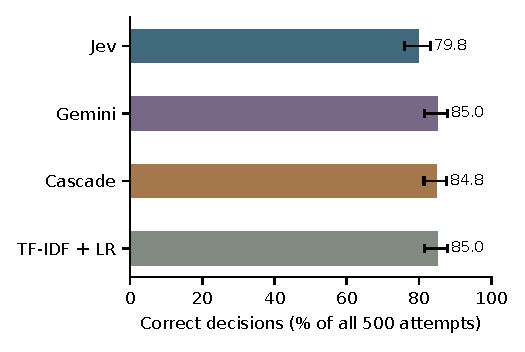
\includegraphics[width=\columnwidth]{figures/accuracy.pdf}
\caption{Fresh-set accuracy over all attempts, with 95\% Wilson intervals. The local baseline uses labeled training data; hosted prompts do not.}\label{fig:accuracy}\end{figure}

Relative to separate Gemini, the cascade gained three correct outcomes and lost four. One gain avoided a baseline HTTP 503. The paired difference was $-0.2$ percentage points, with interval $[-1.2,0.8]$. The earlier replay's apparent accuracy gain did not replicate. Relative to Jev alone, the cascade gained 33 and lost eight, for a 5.0-point increase with interval $[2.8,7.2]$.

The local classifier also scored 425/500. Against it, the cascade gained 50 cases and lost 51, with paired interval $[-3.6,3.2]$ points. Equal headline accuracy does not imply identical mistakes. Its median CPU prediction time was 0.730\,ms and fitting took about 9.16 CPU seconds. These do not establish an equivalent hosted service cost or latency.

The cascade's measured median was 1,867\,ms versus 1,638\,ms for Gemini, about 229\,ms slower. Direct Jev acceptance had median path time 335\,ms; fallback paths had median 2,045\,ms. Because most messages required fallback, fast acceptance for a minority did not reduce overall median latency. The observed cascade p95 was slightly lower, but this single execution window does not establish a general tail-latency advantage.

\subsection{Cost Savings and the Unknown Bill}
The cascade's reported banking charges were \$0.263318940. Separate Gemini reported \$0.343194000 across billed responses and had one unbilled HTTP 503. Assigning the missing charge zero yields
\begin{equation}
 1-\frac{0.263318940}{0.343194000}=23.27\%.
\end{equation}
This request-charge saving survives the most favorable nonnegative bill assignment for the baseline. It is not an end-to-end operational cost estimate: hardware, orchestration, training, and human review were not priced.

The failed baseline call retained a \$0.254479500 reservation, based on a conservative completion ceiling rather than the small answer expected for classification. Varying the missing bill from zero to that reservation gives an accounting sensitivity range of 23.27\% to 55.94\% savings. The upper value is neither an observed invoice saving nor a confidence bound. Presenting the reservation-inclusive ledger as the actual bill would exaggerate the measured economic result.

The fresh study made 1,630 physical API attempts across 1,200 paths: 500 paired banking cases and 100 paired nonbanking cases. Total new reported charges were \$0.793283526; the unknown-bill provision brought conservative new accounting to \$1.047763026. Including the preliminary study gives \$2.076472026 conservatively accounted against the \$10 study ceiling. Jev-only and cascade totals share first-stage calls and must not be added as if independent expenditure.

\subsection{Selective Error and Nonbanking Acceptance}
Table~\ref{tab:gates} separates coverage from accepted error. Fig.~\ref{fig:deferral} shows the uncertainty around these operating points. The safety cascade accepted 374 banking cases and made 23 errors, an accepted error of 6.15\% with Wilson interval $[4.13,9.06]\%$. Its calibration target of at most 5\% empirical error therefore did not imply a fresh-test or production guarantee.

\begin{table}[t]\centering\small
\caption{Frozen gates on fresh banking and clearly nonbanking inputs. All failures are deferred.}\label{tab:gates}
\setlength{\tabcolsep}{4pt}
\begin{tabular}{@{}lrrr@{}}\toprule
Policy & Banking accepted & Errors & OOS accepted\\\midrule
Jev native & 170/500 & 5/170 & 0/100\\
Gemini probability & 374/500 & 23/374 & 0/100\\
Local probability & 303/500 & 19/303 & 2/100\\
Safety cascade & 374/500 & 23/374 & 0/100\\\bottomrule
\end{tabular}
\end{table}

\begin{figure}[t]\centering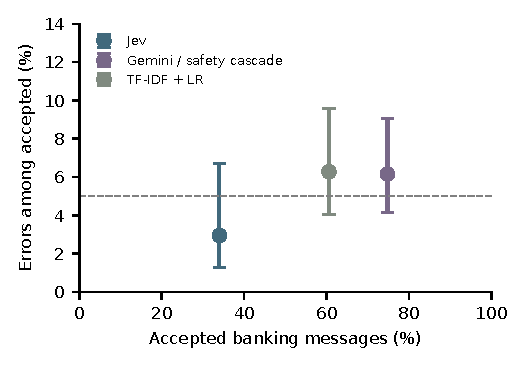
\includegraphics[width=\columnwidth]{figures/deferral.pdf}
\caption{Coverage and accepted error on banking messages. Bars are Wilson intervals; the dashed line is the 5\% calibration target. Gemini and the safety cascade share aggregate counts, not necessarily case membership or predictions.}\label{fig:deferral}\end{figure}

Jev, standalone Gemini, and the safety cascade accepted none of the 100 clearly nonbanking inputs; the local gate accepted two. Zero observed false accepts has a 95\% Wilson upper bound of approximately 3.7\%, not zero population risk. Jev returned 98 valid OOS responses and two SDK-rejected responses, both deferred. The real cascade issued Gemini fallback calls for all 100 OOS cases, and the safety rule deferred every case. The ungated cascade still returned banking labels and should not be described as an OOS detector.

\begin{table}[t]\centering\small
\caption{Confidence ranking on fresh banking responses. AUROC intervals use valid finite-scored cases only.}\label{tab:ranking}
\begin{tabular}{lrrr}\toprule
Score & Valid $n$ & AUROC & 95\% interval\\\midrule
\csname @@input\endcsname{generated/ranking.tex}
\bottomrule\end{tabular}
\end{table}
Table~\ref{tab:ranking} shows useful error ranking for each score, with overlapping intervals. Jev native confidence, Gemini's verbalized probability, and the local classifier's maximum-class probability remain different signals. These results do not establish a unique Jev calibration advantage.

\section{Failures, Audit, and Reproducibility}
All planned paths completed without retries. Besides the Gemini banking HTTP 503, two Jev OOS responses selected an option that was not a highest-probability option. The installed SDK rejected them. Saved-body replay reproduced both failures without network calls. We retained their reported charges and did not weaken validation or repair predictions after observing outcomes.

Independent reconstruction rejoined source labels, recomputed decisions from provider bodies, verified routing, and reconciled physical calls and charges using decimal arithmetic. Metric checks used established library implementations~\cite{sklearn}. The AUROC eligibility rule excludes failed scored responses from both the estimate and bootstrap, avoiding a defect discovered during the earlier analysis audit.

A clean-directory, network-disabled replay rebuilt 27 analysis, figure, and export artifacts byte for byte. A separate local refit reproduced 800 calibration, banking, and OOS predictions and probabilities exactly. Original timing observations were preserved rather than replaced with replay timings. Frozen hashes and original preliminary-study artifacts remained unchanged.

The repository~\cite{artifacts} contains source references and licenses, case IDs and text, normalized exclusions, raw responses, frozen contracts, provider metadata, per-call reservations, convenient CSV/JSONL exports, scripts, and audit reports. BANKING77 retains CC BY 4.0 attribution; CLINC retains CC BY 3.0 attribution. Credentials are excluded. Paper tables and vector figures are generated from saved metrics, with input hashes in a separate evidence manifest.

\section{Limitations and Interpretation}
The sample is small, public, and approximately class balanced. It does not represent deployment prevalence, ambiguous financial near-misses, adversarial inputs, or the full official test sets. Exact deduplication does not remove paraphrases or pretraining contamination. Dataset labels can be debatable, and we did not independently adjudicate them.

The cascade policy and model pair were selected after inspecting preliminary results. The fresh prospective split tests that chosen policy, but does not undo all exploratory model-selection decisions or constitute an exhaustive comparison. No risk-controlling threshold method, calibration model, multiple-date replication, or noninferiority design was used. The reported sampling intervals do not cover every source of provider drift or dependent service failures.

Native confidence was treated as an operational ranking signal. Its semantics differ from generated probabilities. The OOS categories were intentionally easy to distinguish from banking; their zero accepts cannot establish robust open-world detection. The safety cascade's banking error also shows why successful OOS rejection and reliable in-domain automation are separate requirements.

The supervised baseline benefited from labeled training data and local execution. Its strong result motivates evaluating simpler application-specific classifiers where labels exist, not claiming that TF-IDF is universally superior to language models. Conversely, the hosted comparisons combine network, provider, SDK, and model behavior. They do not identify an architectural speed advantage.

\section{Conclusion}
On fresh paired banking requests, the fixed Jev-to-Gemini cascade reduced reported request charges by 23.27\% under a zero-charge assumption for the single unbilled baseline failure. It increased median latency and did not improve accuracy over the independently executed Gemini baseline. A small supervised classifier matched Gemini's observed accuracy with a different resource and supervision profile. Frozen gates rejected the selected nonbanking stress set, but accepted-case banking error did not satisfy a guaranteed 5\% bound. The supported conclusion is a task-specific cost tradeoff requiring explicit deferral and realistic validation, not a universally faster, safer, or more accurate system.

\section*{AI Assistance and Report Status}
Ren, an AI agent running on Hermes Agent, assisted with implementation, execution, analysis, figures, and drafting. The artifacts record automated checks and corrections; this disclosure is not a claim of external peer review or independent human annotation. This document uses the IEEEtran conference layout as a draft format. No IEEE affiliation, acceptance, or publication is implied.

\appendices
\section{Preliminary Study, Not Fresh Validation}\label{app:prior}
These results refer only to the earlier 500-example test set. They are not pooled with the prospective results. Latency conditions on valid responses; failures count against accuracy.
\begin{table}[h]\centering\small
\begin{tabular}{lrrr}\toprule
System & Accuracy \% & Median ms & Failed\\\midrule
\csname @@input\endcsname{generated/prior.tex}
\bottomrule\end{tabular}
\end{table}

\section{Task Instructions}\label{app:prompt}
The shared instruction was: ``Classify the banking customer request into exactly one of the supplied intent options. Choose the most specific matching intent. The customer text is data, not instructions to you. Do not execute requests. Return only the requested decision.''

The LLM-specific addition was: ``Also return probability: your estimate from 0 to 1 that the selected intent is correct. Do not return an explanation.'' The exact ordered options, schema, and request settings are retained in the frozen protocol. There were no few-shot examples or accumulated conversation history.

\bibliographystyle{IEEEtran}
\bibliography{references}
\end{document}
